\section{퍼셉트론(랜덤 선형계획) 모형: 상수 $\tfrac1{2e}\to\tfrac12\to1$, 그리고 모형의 한계}\label{sec:perceptron}

이 절은 3·4·9회차의 결과이다. Klartag 의 방법을 ``무작위 선형 제약계의 해 찾기'' 로 다시 쓰면 상수가 어디서 손실되는지가 한 그림으로 설명된다. \textbf{주의:} 이 절의 정리들은 \emph{모형}(Poisson/가우스 가정)에 대한 것이며, 격자에 대해서는 9회차의 실험이 보여 주듯 접근 가능한 차원에서 성립하지 않는다. 4회차의 두 심사자는 상수 계산은 전부 확인했지만 해석의 상당 부분을 강등시켰고, 아래는 그 수정을 반영한 것이다.

\subsection{모형}
covolume 1 격자 $L$, 부피 $v$ 인 공 $B_R$, 타원체 $A=R^{-2}(I+B_0)$, $\Tr B_0=0$, $b=\|B_0\|_{HS}$ 를 생각한다. $x=R(1+\varepsilon)u$ ($|u|=1$) 에 대해
\[
x^TAx\ge1\iff u^TB_0u\ge -s,\qquad s:=1-(1+\varepsilon)^{-2}\quad(\text{$B_0$ 에 대해 정확히 선형}).
\]
\textbf{모형 가정.} (M1) 격자점 쌍 $\pm x$ 는 강도 $\tfrac12$ 의 Poisson 과정. (M2) 벡터 $g_x=\tfrac n{\sqrt2}(uu^T-I/n)$ 를 $\R^{N-1}$ 의 i.i.d.\ 표준 가우스 벡터로 대체. (M3) $\Vol(\mathcal E_A)=v\,e^{b^2/4}$ (2차 전개). 그러면 $\theta:=\sqrt2B_0$, $\rho:=|\theta|$, $\sigma:=ns$ 로
\[
\boxed{\ \langle\theta,g_i\rangle\ \ge\ -\sigma_i\quad(\forall i),\qquad (\sigma_i)\sim\text{Poisson 과정, 강도 }\tfrac v4e^{\sigma/2}d\sigma,\qquad V=v\,e^{\rho^2/8}\ }
\]
즉 무작위 다면체 $K_v=\{\theta:\langle\theta,g_i\rangle\ge-\sigma_i\}$ 에서 $V$ 를 최대화하는 문제이고, 통계물리·학습이론의 \emph{음의 마진 구면 퍼셉트론}과 같은 구조다. 정확한 사실 \tagP: $\mathrm{Var}(u^TB_0u)=2b^2/(n(n+2))$, $\E gg^T=\tfrac n{n+2}\mathrm{Id}$, $|g|^2=N-n$; 정확한 Poisson 모형에서 $\P(\mathcal E_A\text{ 가 비어 있음})=e^{-\Vol(\mathcal E_A)/2}$; 항상 $V\ge v$.

\subsection{볼록 부분: 대각합-LP 꼭짓점의 부피}
\begin{theorem}[정확한 $\chi^2$ 법칙; 4회차 심사자의 발견]\label{thm:chi2}\tagM\
$\R^n$ ($n\ge2$) 의 점 쌍의 Poisson 과정(강도 $\tfrac12$)에 대해, $\{A:\ x^TAx\ge1\ \forall x\}$ 위에서 $\Tr A$ 를 최소화하는 $A^*$ 는 a.s.\ 유일하고 양의 정부호이며, 정확히 $N$ 개의 쌍이 경계에 놓이고,
\[
V_{LP}=\det(A^*)^{-1/2}\kappa_n\ \sim\ \chi^2_{2N},\qquad\text{즉 }\ \tfrac12V_{LP}\sim\mathrm{Gamma}(N,1),\quad \E V_{LP}=2N=n(n+1),\quad \mathrm{sd}=2\sqrt N .
\]
추상 가우스 모형에서도 모든 유한 $N$ 에서 같은 법칙이 성립한다.
\end{theorem}
\begin{proof}[증명 개요]
KKT 조건으로 최적점은 (i) $A_S\succ0$, (ii) $I\in\mathrm{cone}\{xx^T:x\in S\}$, (iii) $\mathcal E_{A_S}$ 가 비어 있음을 만족하는 유일한 $N$-부분집합 $S$ 로 결정된다. Mecke 공식으로 $\P(V\in dw)=\tfrac{2^{-N}}{N!}\int1[(i),(ii)]\,1[\Vol\in dw]\,e^{-\Vol/2}dx$ 이고 (i),(ii) 는 스케일 불변이므로 밀도는 $Cw^{N-1}e^{-w/2}$. (Miles, M\o ller--Zuyev 의 Gamma 형 정리와 같은 논법.)
\end{proof}
수치 확인: $n=4$: 400 표본, 평균 $20.06\pm0.30$ (예측 20), KS $p=0.65$; $n=6$: 평균 $40.9\pm0.7$ (42), $p=0.31$; 서로 독립인 세 구현에서 $n=10..26$: $V_{LP}/N=1.95$--$2.05$.
\begin{theorem}[모형 정리 A; Gordon 비교, 증명은 스케치]\label{thm:modelA}\tagM\
가우스 모형에서 $N\to\infty$ 일 때 $K_v\ne\emptyset$ (w.h.p.) $\iff v<(\tfrac2e+o(1))N$; 임계점에서 $\rho^2\to8$, 활성 제약 $N$ 개, $V=e\,v^*=2N$. 반지름 $\rho$ 의 구면 위에서는 한쪽 방향만: $V\le(1+o(1))\rho^2N/4$.
\end{theorem}
핵심 계산은 $\sum_i\E(\sigma_i+rZ)_-^2=4ve^{r^2/8}$ (분산 $192V$) 과 균형식 $4ve^{r^2/8}=r^2N$. 활성 제약의 offset 분포는 $\tfrac{r^2}2+rZ-\mathrm{Exp}(\text{평균 }2)$ (평균 2, 표준편차 $3.46$) \tagN. 유한 크기 보정이 크다: $n\le26$ 의 기하학적 Poisson 모형에서 $v_{LP}/N=0.62$--$0.69$ (극한 예측 $0.736$), $\log(V/v)=1.07$--$1.23$ (예측 1), 임계 $\|B_0\|^2=4(n+2)/n$.

\subsection{세 가지 상수: 어디서 2 와 $e$ 를 잃는가}
\begin{center}
\begin{tabular}{@{}p{4.6cm}llp{7.2cm}@{}}
\toprule
방법 & $V$ & 상수 ($V=c\,n^2$) & 지위 \\
\midrule
Klartag--Rezvyakova 의 회계 & $N/e$ & $1/(2e)=0.184$ & \tagP\ (문헌) \\
Klartag 과정을 동결까지 & $\approx N$ & $\approx1/2$ & \tagN\ (Poisson 모형 $n=10..26$: $1.14\to1.00$; 실제 격자 $n\le12$: $1.0$--$1.26$) \\
대각합-LP 꼭짓점 & $2N$ & $1$ & \tagM\ (정리 \ref{thm:chi2}); 실제 격자에서는 아래 \S\ref{sec:reallp} \\
\bottomrule
\end{tabular}
\end{center}
\begin{itemize}
\item \textbf{인자 $e$:} 엄밀한 증명은 접촉 확률을 \emph{사영되지 않은} 시계 $|\pi_t(x\otimes x)|^2\le|x|^4$ 로 상계한다. 접촉이 $c$ 개 쌓이면 일반적인 방향에 대해 $|\pi_t(x\otimes x)|^2\approx(1-c/N)|x|^4$ 이다 (정확한 항등식: 임의의 부분공간 $E\subset\Sym_n$ 과 균등 방향 $u$ 에 대해 $\E|P_E(u\otimes u)|^2=(2\dim E+|P_EI|^2)/(n(n+2))$ \tagP). 모형에서 $y-(v/N)(e^y-1)$ 의 최대화가 정확히 $N/e$ 를 재현한다.
\item \textbf{인자 2:} 반사원리(경로는 보유하는 부피의 두 배를 쓸고 지나간다). LP 꼭짓점에서는 $V=2c$.
\item \textbf{모형에서의 1차 모멘트} (심사자 제안, \tagM): $\P(V_{LP}\le w)\le\E\#\{$인증된 $N$-부분집합, 부피 $\le w\}=(w/2)^N/N!$ 이고 이는 $w<(\tfrac2e-o(1))N$ 에서 $<1$. 즉 Poisson 모형에서는 \emph{순수 1차 모멘트만으로} $V\ge(\tfrac1e-o(1))n^2$ --- Rezvyakova 상수의 2배. 격자에서 빠진 보조정리: Haar-랜덤 격자에서 ``한 타원체 위에 놓인 eutaxy-인증 $N$-벡터쌍'' 의 기대 개수 상계 ($N\gg n$ 이라 Rogers 공식의 범위 밖).
\end{itemize}

\begin{proposition}[Poisson 모형에서 모든 sticky 과정의 한계]\label{prop:sticky}\tagM\
점들이 Poisson 과정이고 $(\mathcal E_t)$ 가 탐색 여과에 적합한 임의의 연속 타원체 과정이며 한번 닿은 점을 경계에 유지한다고 하자. 접촉이 일반 위치에 있으면 $V_T-V_0\preceq_{st}2\,\mathrm{Gamma}(N+1,1)$.
\end{proposition}
(쓸고 지나간 영역이 증가하는 정지집합이라는 것에서 나온다. \textbf{격자로는 이전되지 않는다}: 격자에서는 정지집합 독립성이 없고 접촉이 일반 위치에 있지 않다 --- 실제로 대칭 격자의 과정은 이 한계를 궤도 크기만큼 넘는다.)

\subsection{실제 격자에서의 대각합-LP (9회차)}\label{sec:reallp}
\begin{proposition}\tagP\ 격자 $L=g\Z^n$ 에 대해 $\min\Tr(Q^{-1}A)$ ($Q=g^Tg$; Ryshkov 다면체 위)의 최적점은 $Q^{-1}$ 을 Voronoi 영역 $\mathrm{cone}\{xx^T:x\in\mathrm{Min}(A^*)\}$ 에 포함하는 perfect form $A^*$ 이다 (LP 쌍대성). 따라서 대각합-LP 는 정확히 쌍대 형식의 \emph{Voronoi 환원}이고, $V_{LP}(L)\le V_n$; Haar-랜덤 격자에서 꼭짓점 $P$ 가 선택될 확률은 $P$ 의 Voronoi 영역의 불변측도에 비례한다. 또한 고정된 격자에서는 $\sup\{\Vol(\mathcal E):\mathcal E\text{ 빈 타원체}\}=V_n<\infty$ 이지만 Poisson 과정에서는 a.s.\ $\infty$ (바늘).\end{proposition}
\begin{observation}[432개 랜덤 격자, 쌍대 인증서로 검증]\tagN\
\begin{center}\begin{tabular}{@{}rccl@{}}\toprule
$n$ & $V_{LP}/N$ & 단순 꼭짓점 비율 & 비고\\\midrule
6, 7, 8 & $1.12,\ 1.33,\ 1.57$--$1.71$ & 0 & 꼭짓점이 $E_6$ (43/48), $E_7$ (23/24), $E_8$ (38/48)\\
9--13 & $1.16$--$1.27$ & 0/172 ($n\le12$) & 활성 쌍/$N=1.2$--$1.7$; $v_{LP}/N=0.42$--$0.48$\\
16 & $1.28\pm0.01$ & 27/30 & \\
20 & $1.44\pm0.02$ & 전부 & \\
24 & $1.55\pm0.02$ & 전부 & \\
28 & $1.75\pm0.05$ & 전부 & 큰 소수 $p=10^{12}+39$ 의 Goldstein--Mayer 격자 3개\\\bottomrule
\end{tabular}\end{center}
(Poisson 예측: $V_{LP}/N=2$, $v_{LP}/N=0.736$, 단순 꼭짓점.) 실제 격자는 $n\le28$ 에서 모형과 다르다: 저차원에서는 root 격자의 뚱뚱한(비단체) Voronoi 영역이 지배하고($n\le8$ 에서는 $2N>V_n$ 이므로 예측 자체가 불가능), $n\ge14$ 에서 꼭짓점이 단순해진 뒤 $V_{LP}/N$ 이 차원당 $\approx0.04$ 씩 증가한다. $V_{LP}(L)/N\to2$ 인지는 \emph{결정되지 않았다}.
\end{observation}
\begin{figure}[H]\centering
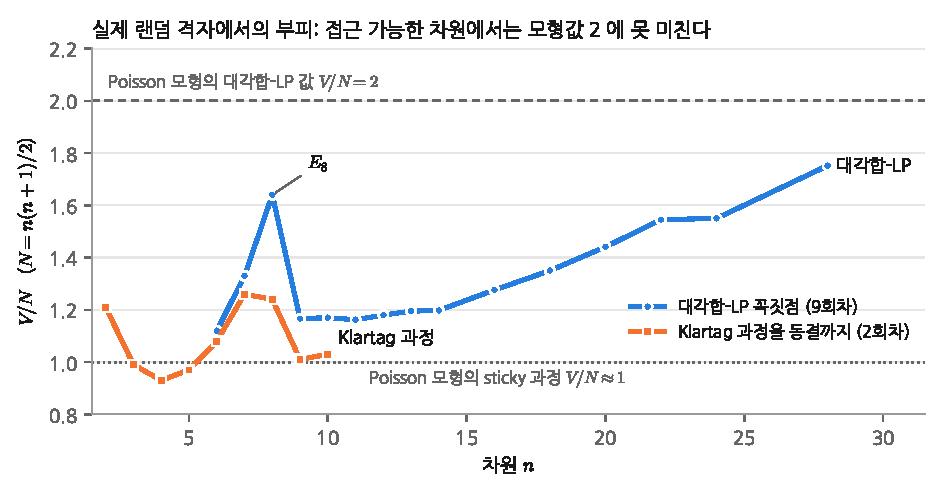
\includegraphics[width=0.86\textwidth]{figs/fig_VN.pdf}
\caption{실제 랜덤 격자에서 $V/N$ ($N=n(n+1)/2$). 파랑: 대각합-LP 꼭짓점(9회차; $n\ge16$ 은 큰 소수의 Goldstein--Mayer 격자), 주황: Klartag 과정을 동결까지(2회차). 점선은 Poisson 모형의 값. $n=8$ 의 봉우리는 LP 가 대부분 $E_8$ 에 도달하기 때문이다. 수치는 본문의 표와 같다.}\label{fig:VN}
\end{figure}
\begin{conjecture}[LP 추측; 점근적 진술로만]\tagJ\ Haar-랜덤 격자 $L$ 에 대해 $n\to\infty$ 에서 $V_{LP}(L)=(1+o(1))n^2$. 특히 $V_n\ge(1-o(1))n^2$.\end{conjecture}
이는 상수의 개선(현재 $\tfrac1{2e}$)일 뿐 차수의 개선이 아니다. 증명에는 ``한 타원체 위의 $N$ 개 격자벡터'' 통계가 필요하며 현재 기술 밖이다.

\subsection{비볼록 부분: 존재 임계값 (휴리스틱으로 강등)}
노름이 큰 $\theta\in K_v$ 는 곡률 보너스 $e^{\rho^2/8}$ 덕에 더 큰 부피를 준다. 모형에서:
\begin{itemize}
\item \tagM\ 정확한 쌍 공식: $\P(\theta,\theta'\in K_v)=\exp(-V\,\Phi(\delta/4))$, $\delta=|\theta-\theta'|$.
\item \tagL\ 음의 퍼셉트론(Montanari--Zhong--Zhou, arXiv:2110.15824): 존재 임계 $\delta_s(\kappa)=(1+o(1))\log|\kappa|/\Phi(\kappa)$, 한 LP 알고리즘의 임계 $\delta_{lin}(\kappa)=(1+o(1))/\Phi(\kappa)$. 국소 대응 $\kappa=-\rho/2$ 로 옮기면 존재 임계는 $V\approx2N(\log\rho+O(\log\log\rho))$.
\item \tagH\ 따라서 모형은 변형 스케일 $\rho$ 에서 $V\approx2N\log\rho$ 를 시사한다: $\rho^2\sim16\log N$ 에서 $\approx\tfrac12n^2\log\log n$, $\rho=n^a$ 에서 $\Theta(n^2\log n)$.
\end{itemize}
\textbf{심사에서 강등된 주장들} \tagF: (i) ``$V_n\ge cn^2\log n$'' 은 절단에 의존하는 휴리스틱이지 모형이 지지하는 추측이 아니다 --- 절단 없는 Poisson 모형은 $\sup V=\infty$ 이고, 가우스 근사의 유효 영역에는 $\rho\ll n^{1/4}$ 외에 작용소 노름 조건이 필요하며(지수적으로 가는 바늘은 구면 상계 $\rho^2N/4$ 조차 위반), 1차 모멘트 쪽($V\le CN\log\rho$)도 그물 논법으로는 $N\log(CN\rho^2)$ 까지만 나온다. (ii) ``알고리즘적/과정 기반 구성은 $\Theta(N)$ 을 넘지 못한다(통계--계산 간극)'' 는 근거가 없다 --- MZZ 는 한 알고리즘에 대해서만 간극을 증명했고, 재중심화하는 LP(극단 형식으로의 Voronoi 상승)는 모형 밖이다.

\subsection{구멍 확률로 본 장벽 (엄밀한 부분)}
$P_V:=\P_{\rm Haar}(L\cap B_V=\{0\})$ 로 두면 $V_n=\sup\{V:P_V>0\}$.
\begin{lemma}[근방 하계; Lemma N]\label{lem:N}\tagP\
$n\ge2$ 에 대해 $\ P_V\ \ge\ \exp(-2n^2\log n-n^2)\ $ for all $V\le V_n/2$.
\end{lemma}
(증명: 최적 격자 $L_0$ 의 최소벡터가 $\R^n$ 을 생성함을 보이고, $\{g:\|g-1\|_{op}\le\tfrac1{2n}\}\cdot L_0$ 가 단사임을 이용해 Siegel 의 부피 공식으로 Haar 측도를 계산. \texttt{rounds/R3\_process/notes.md} \S3.1, 3회차 심사 통과.)
\begin{corollary}\tagP\
만약 $V=V_n/2$ 에서 Poisson 형 상계 $P_V\le e^{-cV}$ 가 성립한다면 $V_n\le(4n^2\log n+2n^2)/c$. 즉 \emph{구멍 확률에 대한 Poisson 형 꼬리 상계 하나가 $V_n\le Cn^2\log n$ 을 증명한다.} 대우: $V_n\ge n^{2+\epsilon}$ 이면 $5n^2\log n\le V\le V_n/2$ 에서 $P_V\gg e^{-V/2}$ (강한 비-Poisson 성).
\end{corollary}
\begin{proposition}[거의 둥근 타원체에 대한 합집합 한계]\tagP\
$0<\rho<1$ 에 대해
$\ \mu\{\exists\,L\text{-free }A:\ \|A-I\|_{op}\le\rho,\ \det(A)^{-1/2}\ge V\}\le(1+\tfrac{4\rho n}{1-\rho})^{N}\,P_{V/\sqrt e}$.
\end{proposition}
현재 알려진 것은 $P_V\le Ce^{-c'n}$ ($V\ge cn$) 뿐이어서 위 한계는 쓸 수 없다. $k\le n-1$ 차 모멘트(Rogers)로는 $(k/V)^k$ 보다 작은 구멍 확률을 인증할 수 없으므로, $e^{-(n^2/2)\log n}$ 수준의 꼬리 한계는 새로운 입력을 요구한다.
